% !TEX root = Main.tex
%\section{Missing Proofs from Section~\ref{Sec:GraphFamilies}}\label{App:GraphFamilies}
%\subsection{Proof of Lemma~\ref{prop:powerlawsparse}}
%By Proposition \ref{prop:maxvertexproper}, the maximum degree of an $n$-vertex $\alpha$-proper power-law
%graph is at most $k' \triangleq \left(\frac{C}{\alpha - 1} + 2\right) \sqrt[\alpha]{n} + 2$, whence
%the total number of edges is at most $\frac{1}{2}\sum_{k=1}^{k'} k \vert V_k\vert$. By definition,
%$\vert V_k \vert\leq \lceil \frac{Cn}{k^\alpha}\rceil \leq \frac{Cn}{k^{\alpha}} + 1$, and thus
%\begin{align*}
%\frac{1}{2}\sum_{k=1}^{k'} k\vert V_k\vert &\leq \frac{1}{2}\sum_{k=1}^{k'} k \left(\frac{Cn}{k^{\alpha}} + 1 \right)
% \leq \frac{k'(k'+1)}{4} + Cn\sum_{k=1}^{\infty} k^{-\alpha+1} \\
%&   = O(n^{2/\alpha}) + Cn \zeta(\alpha - 1) = O(n).
%\end{align*}
%
%\subsection{Proof of Lemma~\ref{prop:Contained}}
%Let $d = \lfloor(\frac C{\alpha - 1} + 2)\sqrt[\alpha]{n} + 2\rfloor$. For any $\alpha$-proper power-law graph with $n$ vertices and for any $k$, $\vert V_k\vert\leq Ck^{-\alpha}n + 1$ and by Proposition~\ref{prop:maxvertexproper}, $\vert V_k\vert = 0$ when $k > d$.
%
%Let $k$ be an arbitrary integer between $\sqrt[\alpha]{n/\log n}$ and $n-1$. We need to show that $\sum_{i = k}^{n-1} {\vert V_i\vert} \leq C'(\frac{n}{k^{\alpha-1}})$. It suffices to show this for $k\leq d$. We have
%\begin{align*}
%  \sum_{i = k}^{n-1} {\vert V_i\vert} & \leq \sum_{i = k}^d(Ci^{-\alpha}n + 1)
%    =    d - k + 1 + Cn\sum_{i = k}^d i^{-\alpha}\\
%  & \leq (\frac C{\alpha - 1} + 2)\sqrt[\alpha]{n} + 3 - k + Cn\int_k^d x^{-\alpha}dx\\
%  & \leq (\frac C{\alpha - 1} + 4)\sqrt[\alpha]{n} + Cn\left[\frac 1{\alpha - 1}x^{-\alpha+1}\right]_\infty^k\\
%  & \leq ((\frac C{\alpha - 1} + 4)(\frac{\sqrt[\alpha]nd^{\alpha-1}}n) + \frac {C}{\alpha - 1})nk^{-\alpha +1}\\
%  & \leq ((\frac C{\alpha - 1} + 4)(\frac C{\alpha-1} + 4)^{\alpha - 1} + \frac{C}{\alpha - 1})nk^{-\alpha+1} \leq C'nk^{-\alpha+1},
%\end{align*}
%as desired.

%\section{Missing Proofs from Section~\ref{Sec:ScaleFree}}\label{App:ScaleFree}
%\subsection{Proof of Lemma~\ref{Lemma:Relations}}
%We first claim that an optimal labeling scheme for the family $\la$ will give the same labeling assignment to any two isomorphic graphs $G_1$ and $G_2$.
%From this it follows that ${{N}\choose{n}} \geq \vert \mathcal{F}_n \vert$.
%
%A  $\log \vert \mathcal{F}_n \vert+ \log n$ labeling scheme for $\mathcal{F}_n$ is achieved in the following way.
%We first assign each graph $G=(V,E)$ a unique identifier using at most  $\log \vert \mathcal{F}_n \vert$ bits.
%A vertex $v \in V$ receives a label that is a concatenation of a unique ID for $v$ and the unique identifier of $G$.
%
%\subsection{Proof of Proposition~\ref{Th:baLabeling}}


\newpage
\section{Experimental results in detail}\label{App:ExpRes}
Subsections ~\ref{App:ExpRes:MaxLabelSyn} and \ref{App:ExpRes:MaxLabelEmp}  show the maximum label sizes for all synthetic and real-world data sets, respectively.
%Section~\ref{Section:DataSetsFull} provides a full description of the data sets and Section~\ref{Section:TableInDetail}  contains the table of  label sizes  for different labeling schemes in full detail.

\subsection{Maximum label size distribution for synthetic datasets}\label{App:ExpRes:MaxLabelSyn}
\begin{figure}[!ht]
\centering
\subfloat[\small syn300$^{\alpha=2.2}$]{
    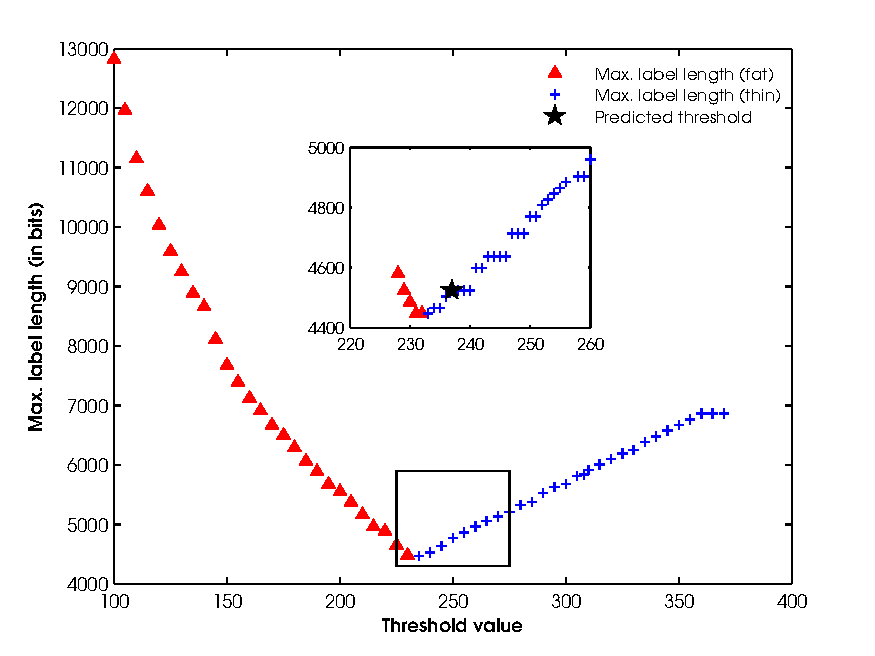
\includegraphics[width=0.5\textwidth]{Figures/synthetic-300k-alpha22.pdf}
}
\subfloat[\small syn300$^{\alpha=2.4}$]{
    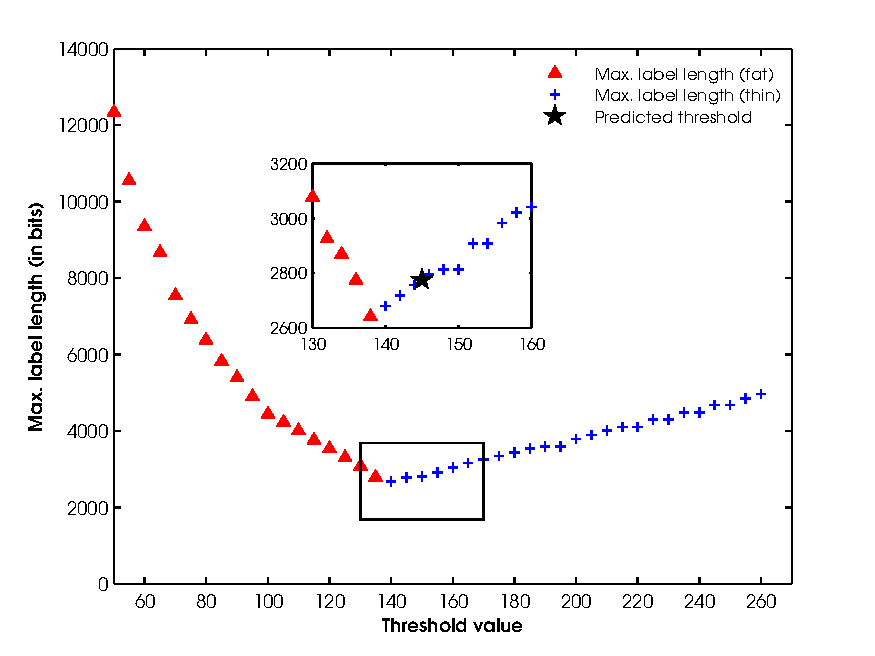
\includegraphics[width=0.5\textwidth]{Figures/synthetic-300k-alpha24.pdf}
}%
\quad
\subfloat[\small syn300$^{\alpha=2.6}$]{
    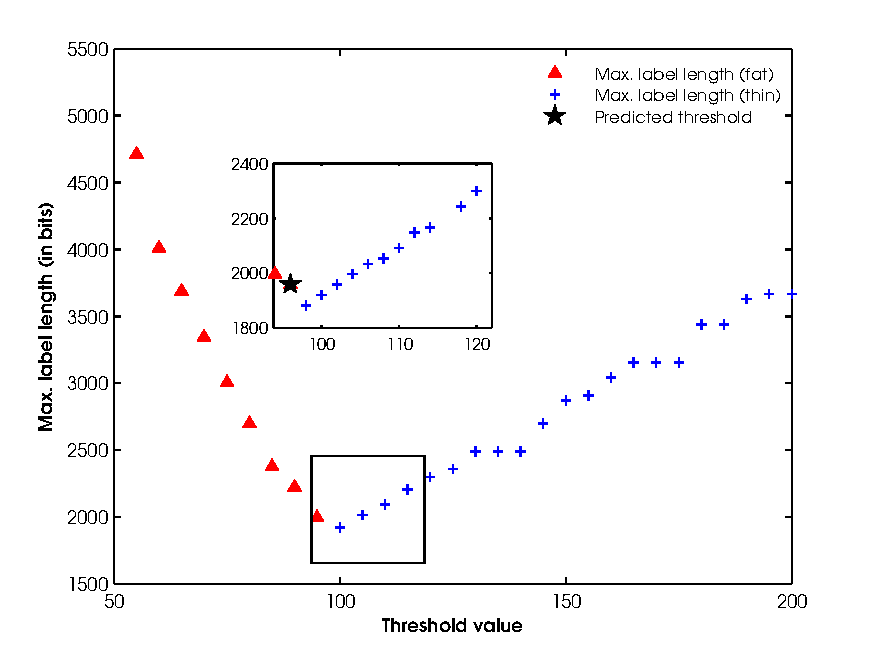
\includegraphics[width=0.5\textwidth]{Figures/synthetic-300k-alpha26.pdf}
}
\subfloat[\small syn300$^{\alpha=2.8}$]{
    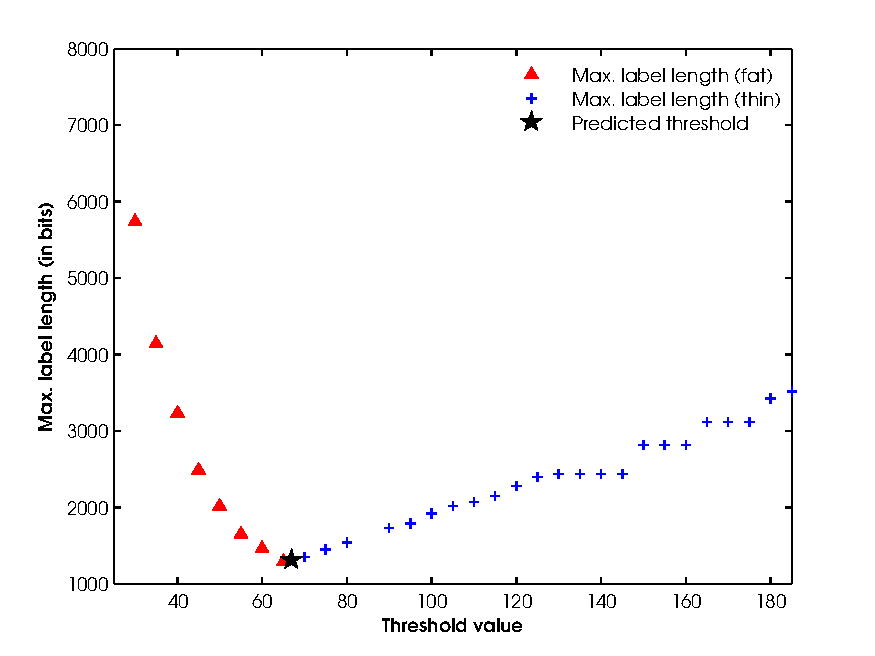
\includegraphics[width=0.5\textwidth]{Figures/synthetic-300k-alpha28.pdf}
}%
\caption{Distribution of maximum label sizes for four different synthetic datasets of $\vert V\vert = 300,000$. Each dataset was generated using one of $\alpha$-values: $2.2,~2.4,~2.6,~2.8$. Fat vertices are shown as red triangles and thin vertices as blue crosses. The black pentagram shows the label size obtained by using the \emph{predicted} threshold. The transition between fat and thin vertices is the maximum label size obtained by using the empirical threshold.}%
\label{fig:synthetic300}%
\end{figure}


\begin{figure}[!ht]
\centering
\subfloat[\small syn1M$^{\alpha=2.4}$]{
    \includegraphics[width=0.5\textwidth]{Figures/synthetic-1m-24.pdf}
}%
\subfloat[\small syn1M$^{\alpha=2.6}$]{
    \includegraphics[width=0.5\textwidth]{Figures/synthetic-1m-26.pdf}
}
\quad
\subfloat[\small syn1M$^{\alpha=2.8}$]{
    \includegraphics[width=0.5\textwidth]{Figures/synthetic-1m-28.pdf}
}%
\caption{Distribution of maximum label sizes for three different synthetic datasets of $\vert V\vert = 1,000,000$. Each dataset was generated using one of $\alpha$-values: $2.4,~2.6,~2.8$. Fat vertices are shown as red triangles and thin vertices as blue crosses. The black pentagram shows the label size obtained by using the \emph{predicted} threshold. The transition between fat and thin vertices is the maximum label size obtained by using the empirical threshold.}%
\label{fig:synthetic1M}%
\end{figure}
\clearpage

\subsection{Maximum label size distribution for real-life datasets}\label{App:ExpRes:MaxLabelEmp}
For completeness,  we  provide an illustration of the best-fitting power law fitted to the probability mass function of the data.


\begin{figure}[!ht]
\centering
\subfloat[\small Fat and thin vertices vs. threshold values]{
    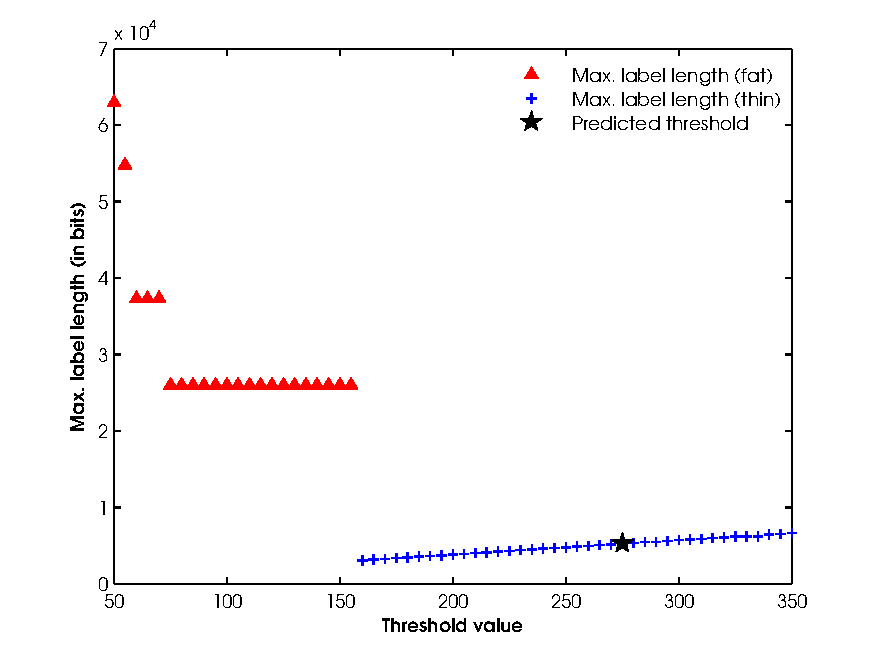
\includegraphics[width=0.5\textwidth]{Figures/barabasi-www.pdf}
}%
\subfloat[\small Power law fit]{
    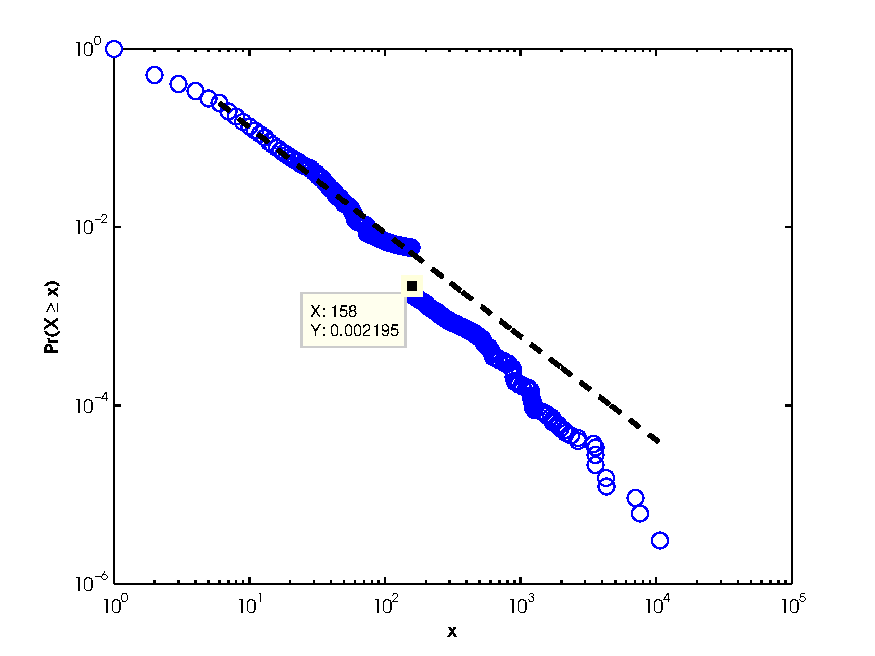
\includegraphics[width=0.5\textwidth]{Figures/barabasi-www-ccdf.pdf}
}%
\caption{Left: Fat and thin vertices plotted against increasing threshold values for the \textsc{www} dataset. The black pentagram shows the predicted threshold ($1/\zeta(\alpha)\sqrt[\alpha](n)$) rounded to nearest integer. Right: Best-fitting power law ($\alpha = 2.16$) superimposed on the complementary cumulative distribution function (CCDF) using the framework by \cite{clauset2009power}.} %
\label{fig:www}%
\end{figure}

\begin{figure}[!ht]
\centering
\subfloat[\small Fat and thin vertices vs. threshold values]{
    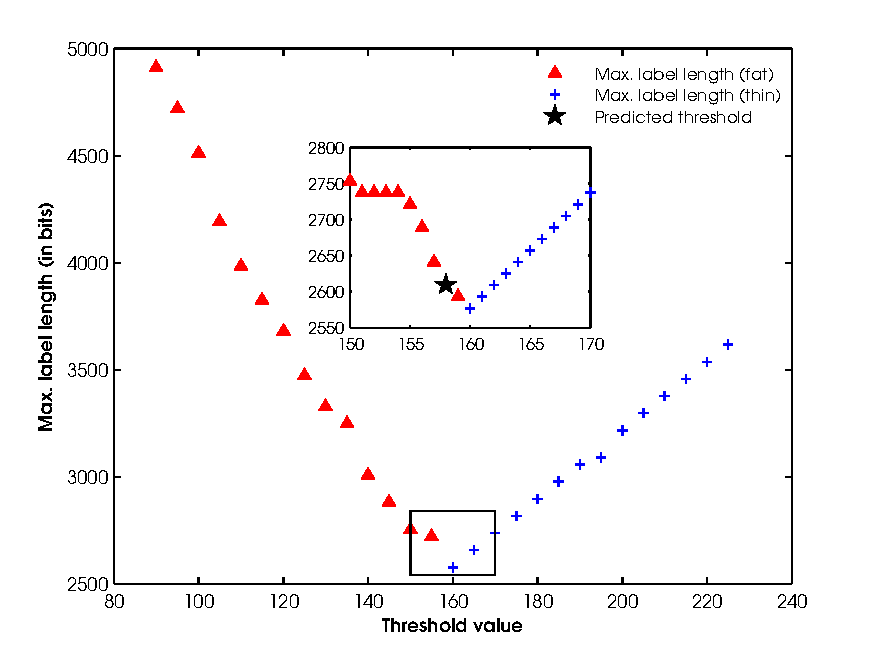
\includegraphics[width=0.5\textwidth]{Figures/enron-mail.pdf}
}%
\subfloat[\small Power law fit]{
    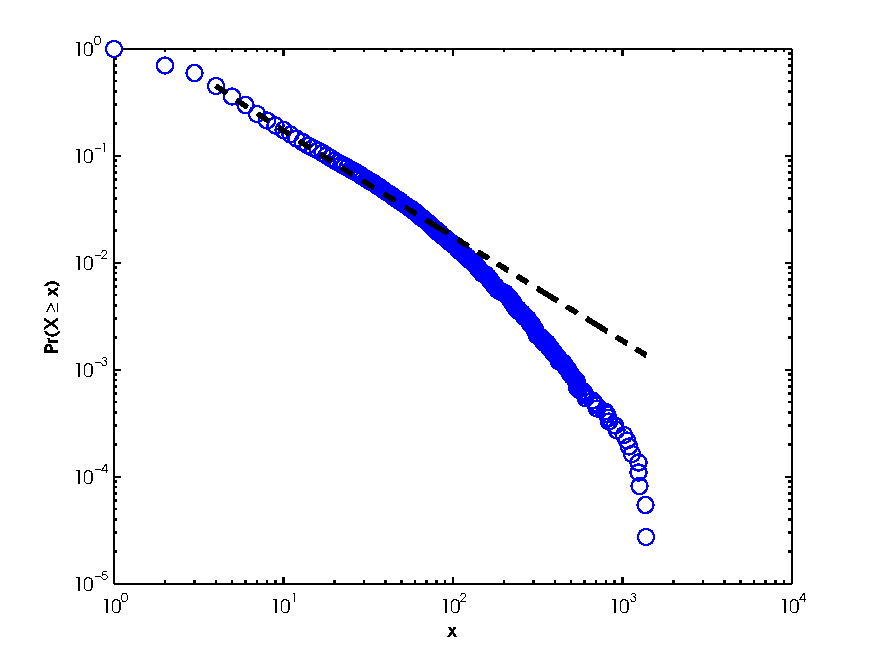
\includegraphics[width=0.5\textwidth]{Figures/enron-mail-ccdf.pdf}
}%
\caption{Left: Fat and thin vertices plotted against increasing threshold values for the \textsc{enron} email communication dataset. The black pentagram is the predicted threshold ($1/\zeta(\alpha)\sqrt[\alpha](n)$) rounded to the nearest integer. Right: Right: Best-fitting power law ($\alpha = 1.97$)  superimposed on the complementary cumulative distribution function (CCDF) using the framework by \cite{clauset2009power}.}
\label{fig:enron}%
\end{figure}

\begin{figure}[!ht]
\centering
\subfloat[\small Fat and thin vertices vs. threshold values]{
    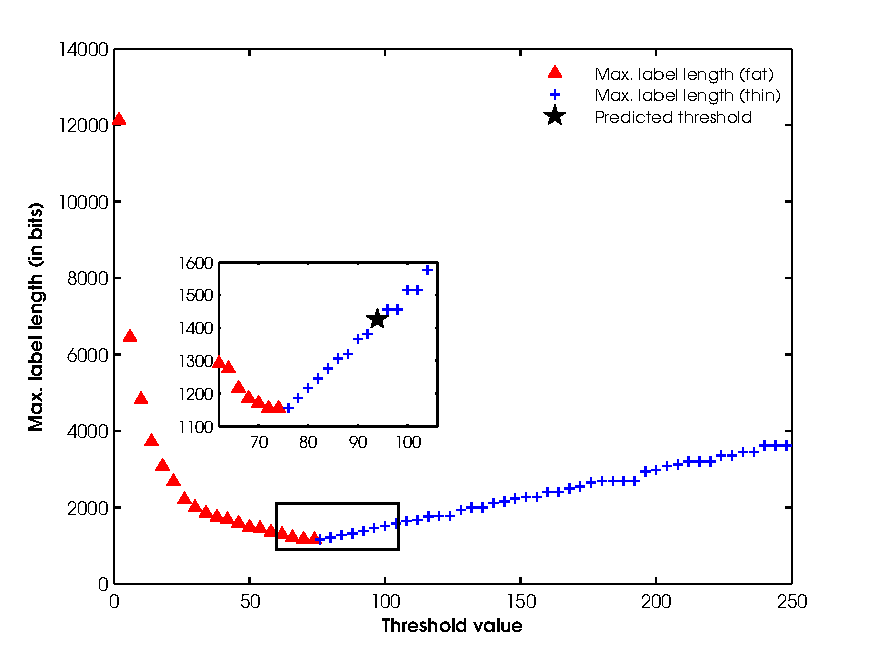
\includegraphics[width=0.5\textwidth]{Figures/internet.pdf}
}%
\subfloat[\small Power law fit]{
    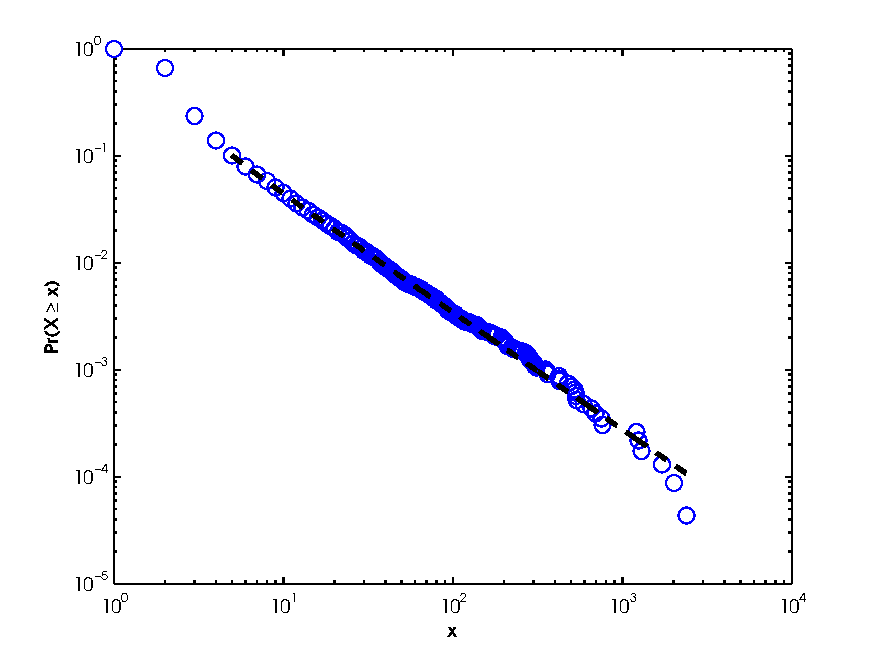
\includegraphics[width=0.5\textwidth]{Figures/internet-ccdf.pdf}
}%
\caption{Left: Fat and thin vertices plotted against increasing threshold values for the \textsc{internet} dataset. The black pentagram is the predicted threshold ($1/\zeta(\alpha)\sqrt[\alpha](n)$) rounded to nearest integer. Right: Right: Best-fitting power law ($\alpha = 2.09$) superimposed on the complementary cumulative distribution function (CCDF) using the framework by \cite{clauset2009power}.} %
\label{fig:internet}%
\end{figure}

%
%\subsection{A full description of the data sets} \label{Section:DataSetsFull}
%The following table includes the number of vertices, edges, $\alpha$ value and maximum degree for each of the data sets.
%\begin{table}[!ht]
%\centering
%\small
%\begin{tabular}{lccccl}\hline
%\multicolumn{6}{c}{Real-Life}\\\hline
%Dataset  & $\vert V \vert$ & $\vert E\vert$ & $\alpha$  & $\Delta_{max}$ & Source\\\hline
%\textsc{www}      & 325,729        & 1,117,563     & 2.16 & 10,721            & \cite{albert1999internet}\\
%\textsc{enron}    &  36,692        &   183,830      & 1.97    &1,383         & \cite{leskovec2009community}\\
%\textsc{internet} &  22,963        &    48,436      & 2.09     & 2,390        & \cite{newman}\\\hline
%
%\multicolumn{6}{c}{Synthetic}\\\hline
%s1M$^{\alpha=2.4}$    & 1,000,000       & 1,127,797      & 2.4    & 42,683 &-- \\
%s1M$^{\alpha=2.6}$    & 1,000,000       & 878,472        & 2.6    & 12,169 &-- \\
%s1M$^{\alpha=2.8}$    & 1,000,000       & 751,784         & 2.8   & 1,692  &-- \\
%s300$^{\alpha=2.2}$    & 300,000        & 491,926        & 2.2    & 10,906 & --\\
%s300$^{\alpha=2.4}$    & 300,000        & 327,631        & 2.4    & 3,265 & --\\
%s300$^{\alpha=2.6}$    & 300,000        & 261,949        & 2.6    & 1,410 & --\\
%s300$^{\alpha=2.8}$    & 300,000        & 227,247        & 2.8    & 1,842 & --\\\hline
%\end{tabular}
%\caption{Datasets and their properties. All graphs are undirected and simple. $\Delta_{max}$ stands for the maximum degree amongst the graph's nodes.}
%\label{t:datasets}
%\end{table}
%
%
%\subsection{Table~\ref{t:labelsizes} in full detail}\label{Section:TableInDetail}
%The following extends Table~\ref{t:labelsizes}  in full detail and   describes the maximum label sizes achieved using different labeling schemes on \emph{all} our data sets. 
%We remind the reader that ``Predicted'' shows the experimental maximum label size obtained by running our scheme on the graphs, ``Empirical'' is the label size attained by using the empirical threshold. The remaining columns show non-experimental upper bounds for different label schemes: ``Bound'' is the upper bound guaranteed in Proposition~\ref{prop:labelingMain}, ``$C$-sparse'' is  the $\sqrt{2cn}+\log n+1$ labeling   defined in Proposition~\ref{sparse-label}'' with simple concatenation of labels to represent the fat bit string, ``BD'' is the $\lceil \frac{\Delta}{2} \rceil \lceil \log n\rceil$ bounded degree graph  labeling of~\cite{adjiashvili2014labeling}, and AKTZ is the $\lceil n/2\rceil+6$ general graph  labeling of~\cite{alstrup2014adjacency}.
% 
%\begin{table}[!h]
%\centering
%\small
%\begin{tabular}{l|llllll}
%Dataset             & Predicted & Empirical & Bound     &$C$-sparse & BD       & AKTZ \\\hline
%s1M$^{\alpha=2.4}$  &$4,841$    &$4,821$    & $19,873 $ &$30,060$   &$426,820$ &$500,006$\\\hline
%s1M$^{\alpha=2.6}$  &$3,361$    &$3,201$    & $12,642 $ &$26,540$   &$121,680$ &$500,006$\\\hline
%s1M$^{\alpha=2.8}$  &$2,101$    &$2,061$    & $8,583 $  &$24,560$   &$16,920$  &$500,006$\\\hline
%s300$^{\alpha=2.2}$ &$4,523$    &$4,447$    & $17,938 $ &$18,867$   &$103,607$ &$150,006$\\\hline
%s300$^{\alpha=2.4}$ &$2,775$    &$2,680$    & $10,996 $ &$15,409$   &$31,008$  &$150,006$\\\hline
%s300$^{\alpha=2.6}$ &$1,958$    &$1,920$    & $7,276 $  &$13,775$   &$13,395$  &$150,006$\\\hline
%s300$^{\alpha=2.8}$ &$1,350$    &$1,312$    & $5,106 $  &$12,844$   &$17,499$  &$150,006$\\\hline
%\textsc{www}        &$5,245$    &$3,060$    & $20,912 $ &$28,443$   &$101,840$ &$162,870$ \\\hline
%\textsc{enron}      &$2,609$    &$2,577$    & $10,243 $ &$9,728$    &$11,056$  &$18,352$\\\hline
%\textsc{internet}   &$1,426$    &$1,156$    & $5,706 $  &$4,575$    &$17,925$  &$11,487$\\\hline 
%\end{tabular}
%\caption{Maximum label sizes for different labeling scheme. See description above.}
%\label{App:t:complabelschemes}
%\end{table}
%% Casper- I got the values 19449 WWW, 6682 ENRON, 3436 INTERNET, 21042 s1m2.4, 18572 2.6, 17182 2.8, 12909 s1m2.2, 12909 2.4, 10538 2.6, 9424 2.6, 8779 2.8.  I wonder why we got different results, 
%%I used 
%function r = Csparse(v,e)
%    c= e/v
%    sparse = sqrt(2*c*v)*ceil(log(v))+ ceil(log(v))+1
%    r=ceil(sparse);

%\begin{table}[!ht]
%\centering
%\small
%\begin{tabular}{l|llllll}
%Dataset             & Predicted & Empirical & Bound     &$C$-sparse & BD       & AKTZ \\\hline
%s1M$^{\alpha=2.4}$  &$4,841$    &$4,821$    & $8,270 $  &$6,746$   &$426,820$ &$500,006$\\\hline
%s1M$^{\alpha=2.6}$  &$3,361$    &$3,201$    & $5,798 $  &$5,959$   &$121,680$ &$500,006$\\\hline
%s1M$^{\alpha=2.8}$  &$2,101$    &$2,061$    & $4,280 $  &$5,516$   &$16,920$  &$500,006$\\\hline
%s300$^{\alpha=2.2}$ &$4,523$    &$4,447$    & $6,950 $  &$4,269$   &$103,607$ &$150,006$\\\hline
%s300$^{\alpha=2.4}$ &$2,775$    &$2,680$    & $4,763 $  &$3,491$   &$31,008$  &$150,006$ \\\hline
%s300$^{\alpha=2.6}$ &$1,958$    &$1,920$    & $3,463 $  &$3,125$   &$13,395$  &$150,006$\\\hline
%s300$^{\alpha=2.8}$ &$1,350$    &$1,312$    & $2,638 $  &$2,914$   &$17,499$  &$150,006$\\\hline
%\textsc{www}        &$5,245$    &$3,060$    & $7,880 $  &$6,436$   &$101,840$ &$162,870$ \\\hline
%\textsc{enron}      &$2,609$    &$2,577$    & $3,741 $  &$2,393$    &$11,056$  &$18,352$\\\hline
%\textsc{internet}   &$1,426$    &$1,156$    & $2,313 $  &$1,215$    &$17,925$  &$11,487$\\\hline 
%\end{tabular}
%\caption{\textcolor{red}{CP: Please write something here}}
%\label{App:t:complabelschemes}
%\end{table}

%
%\section{The impact of the labeling scheme on the total storage}\label{Section:TotalStorage}
%In these   experiments, we measure the overhead caused by our labeling scheme to the total number of bits required to store the graph. We compare  $\textrm{EMP}(G,\tau)$---the total 
%number of bits used by all labels assigned to $G$ with threshold $\tau$---to $\textrm{CENT}(G)$---the total number of bits needed to represent $G$ in a standard, centralized adjacency list. In general, the ratio $\textrm{RATIO}(G,\tau) = \textrm{EMP}(G,\tau)/\textrm{CENT}(G)$ will be greater than $1$ due to the overhead incurred by distributed storage
%of adjacency; for example, na\"{i}vely storing the bit vector of adjacent vertices  in the label of each vertex would
%yield $\textrm{RATIO}(G,\tau) \sim n^2$, whereas our labeling scheme ensures that $\textrm{RATIO}(G,\tau) \sim n\sqrt[\alpha]{n}\log(n)$ for power-law graphs. Low values of $\textrm{RATIO}(G,\tau)$ mean that this overhead is also small for actual networks, whose degree distribution may only approximately follow a power law.
%
%The total storage needed to represent the graph is quite easy to measure:
%Given the $n$ vertex graph $G=(V,E)$ and our labeling scheme $\la$, let $CENT(G)$ be the number of bits required to store the graph in a non-distributed adjacency list form. Given a threshold $\tau$, let $EMP(G,\tau)$ be the sum of the size of all label assignments given to $G$ by $\la$ with threshold $=\tau$. We define $RATIO(G,\tau) = EMP(G,\tau)/ CENT(G)$. Note that $1 \leq EMP(G,\tau)/ CENT(G) \leq 2$. We show the values of $RATIO(G,\tau)$ for the syn$^{\alpha=2.2}$ dataset in Figure \ref{fig:ratiosyn30022}.
%For this data set, $\vert V \vert = 300,000$ vertices and $\vert E \vert= 491,926$ edges, and thus:
%$$ CENT(G) = (\vert E \vert+\vert V \vert) \lceil \log{\vert V \vert} \rceil  = 15,046,594,$$
%And:
%$$ EMP(G,0) =  EMP(G,\Delta(G))  = (2\vert E \vert+\vert V \vert) \lceil \log{\vert V \vert} \rceil + {\vert V \vert}=24,693,188, $$
%where $\Delta(G)$ is the largest degree in $G$.
% We see that  $RATIO(G,0 ) = RATIO(G,\Delta(G) ) = 1.641$ as seen in Figure~\ref{fig:ratiosyn30022}.
%Note that our labeling scheme can be transformed so that $RATIO(G,\tau)=1$ for all $\tau$ simply by orienting the edges of the graph, including edges between two fat or two thin vertices.
%$RATIO(G,\tau)$ can thus be considered as a comparative measurement for the number of bits saved by our labeling scheme alone.
%
%\begin{figure}[!ht]
%\centering
%\subfloat[\small $RATIO(G,\tau)$ for threshold values (in steps of 50) smaller than $\tau=1000$]{
%    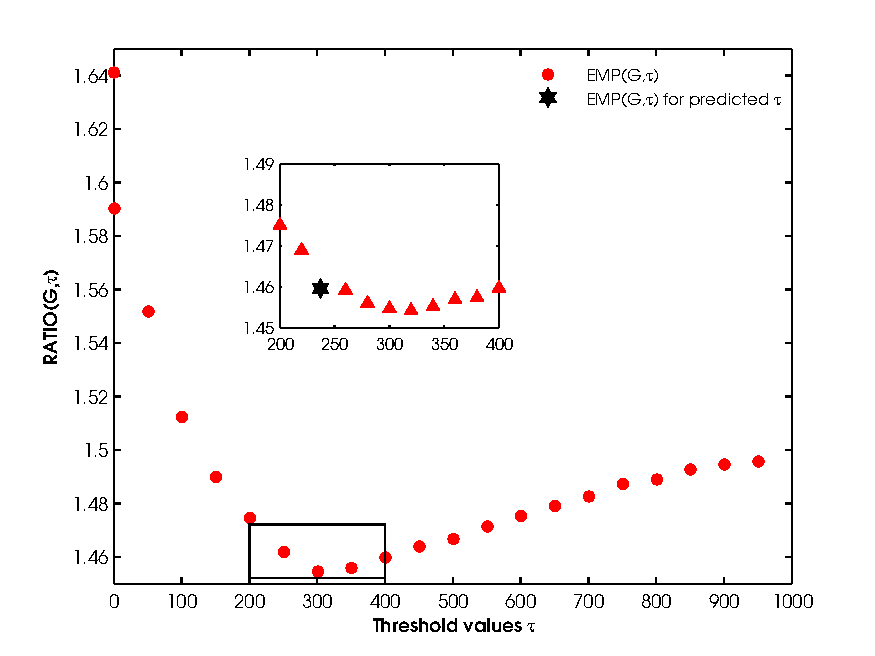
\includegraphics[width=0.45\textwidth]{Figures/synthetic-300k-22-ratio.pdf}
%}
%\quad
%\subfloat[\small $RATIO(G,\tau)$ for selected threshold values covering the range of $\tau$]{
%    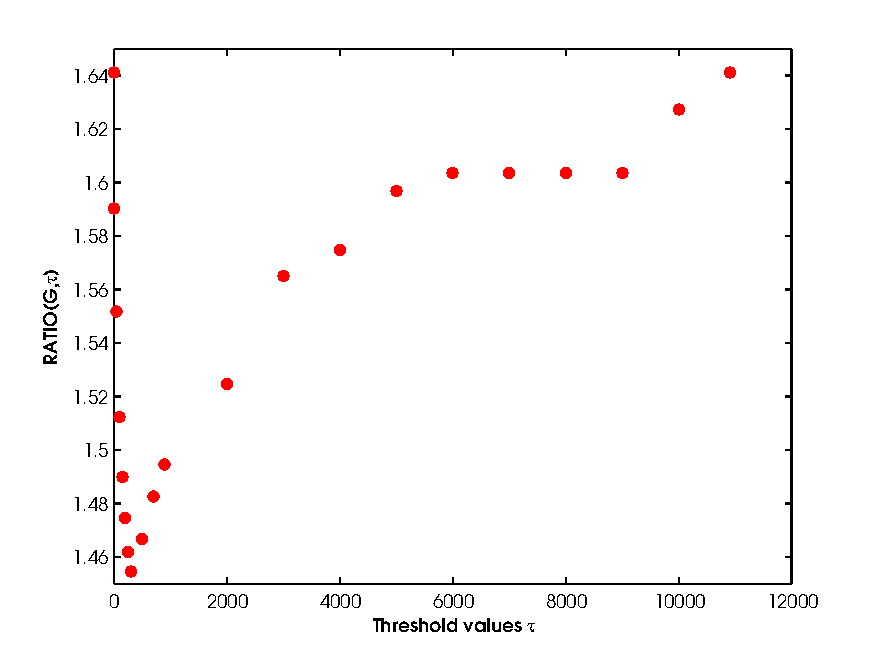
\includegraphics[width=0.45\textwidth]{Figures/synthetic-300k-22-ratio-allrange.pdf}
%}%
%\caption{$RATIO(G,\tau)$ for syn$^{\alpha=2.2}$}
%\label{fig:ratiosyn30022}%
%\end{figure}
%
%\begin{figure}[!ht]
%\centering
%\subfloat[\small syn1M$^{\alpha=2.4}$]{
%    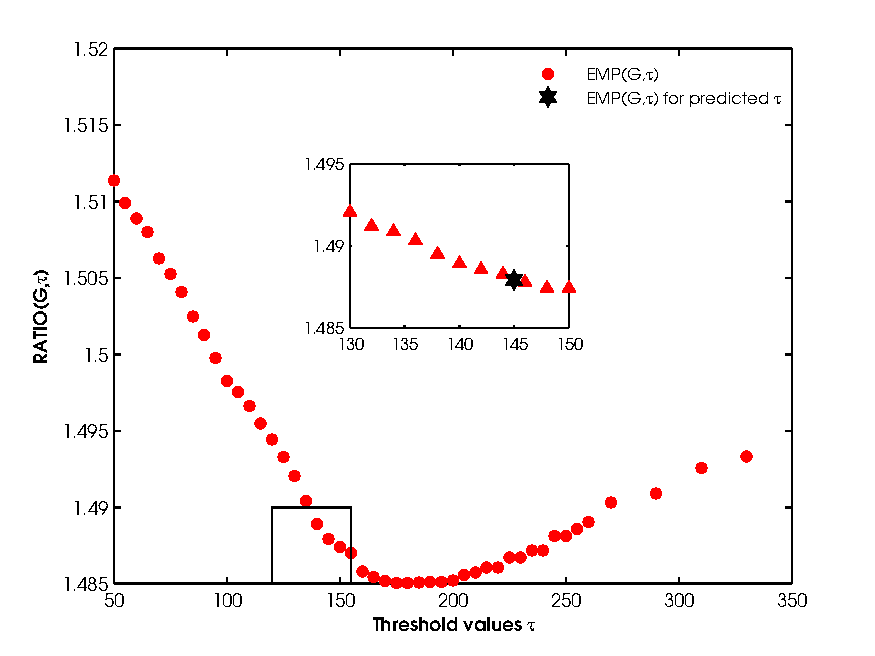
\includegraphics[width=0.5\textwidth]{Figures/synthetic-300k-24-ratio.pdf}
%}%
%\subfloat[\small syn1M$^{\alpha=2.6}$]{
%    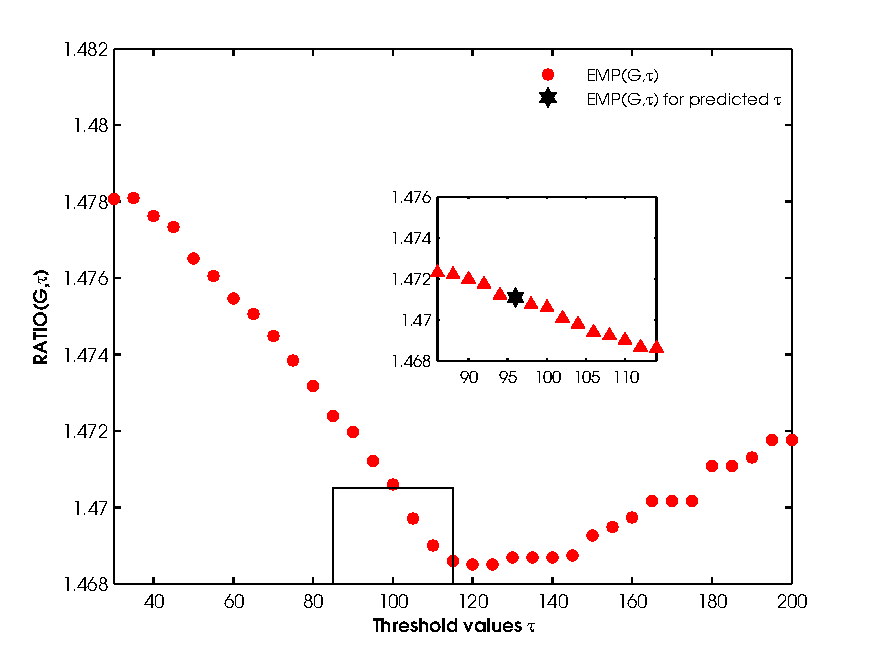
\includegraphics[width=0.5\textwidth]{Figures/synthetic-300k-26-ratio.pdf}
%}
%\quad
%\subfloat[\small syn1M$^{\alpha=2.8}$]{
%    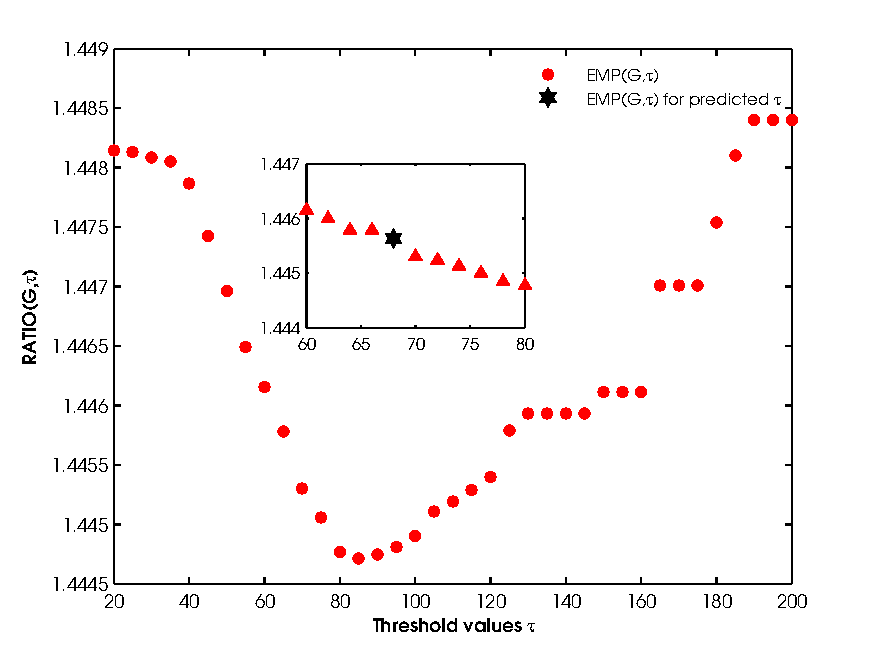
\includegraphics[width=0.5\textwidth]{Figures/synthetic-300k-28-ratio.pdf}
%}%
%\subfloat[\small syn1M$^{\alpha=2.4}$]{
%    \includegraphics[width=0.5\textwidth]{Figures/synthetic-1m-24-ratio.pdf}
%}%
%\quad
%\subfloat[\small syn1M$^{\alpha=2.6}$]{
%    \includegraphics[width=0.5\textwidth]{Figures/synthetic-1m-26-ratio.pdf}
%}
%\subfloat[\small syn1M$^{\alpha=2.8}$]{
%    \includegraphics[width=0.5\textwidth]{Figures/synthetic-1m-28-ratio.pdf}
%}%
%
%\caption{Ratios for synthetic 1M sets}%
%\label{fig:synthetic300Kratios}%
%\end{figure}
%\clearpage
%
%\begin{figure}[!ht]
%\centering
%\subfloat[\small \textsc{www}]{
%    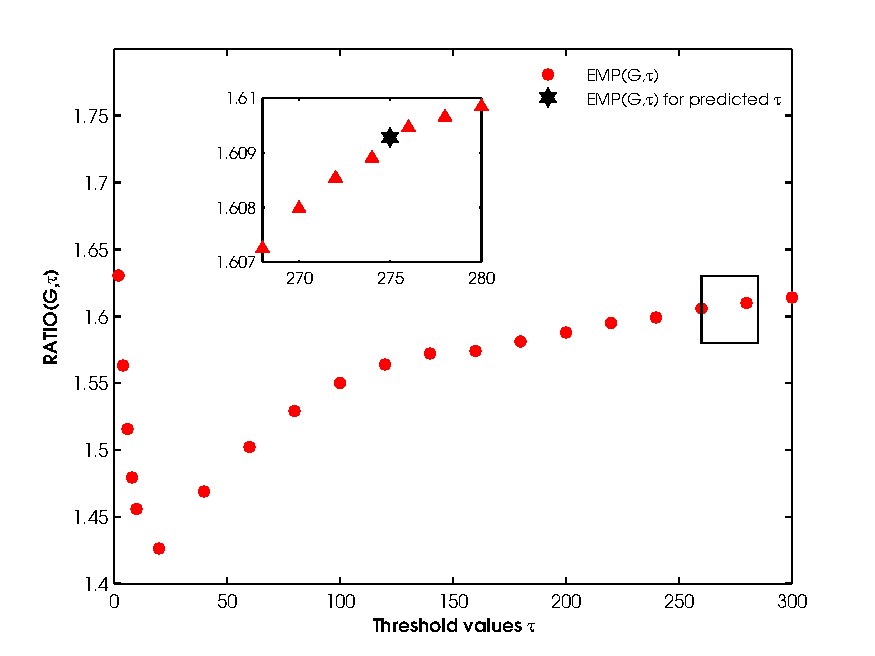
\includegraphics[width=0.5\textwidth]{Figures/www-ratio.pdf}
%}%
%\subfloat[\small \textsc{enron}]{
%    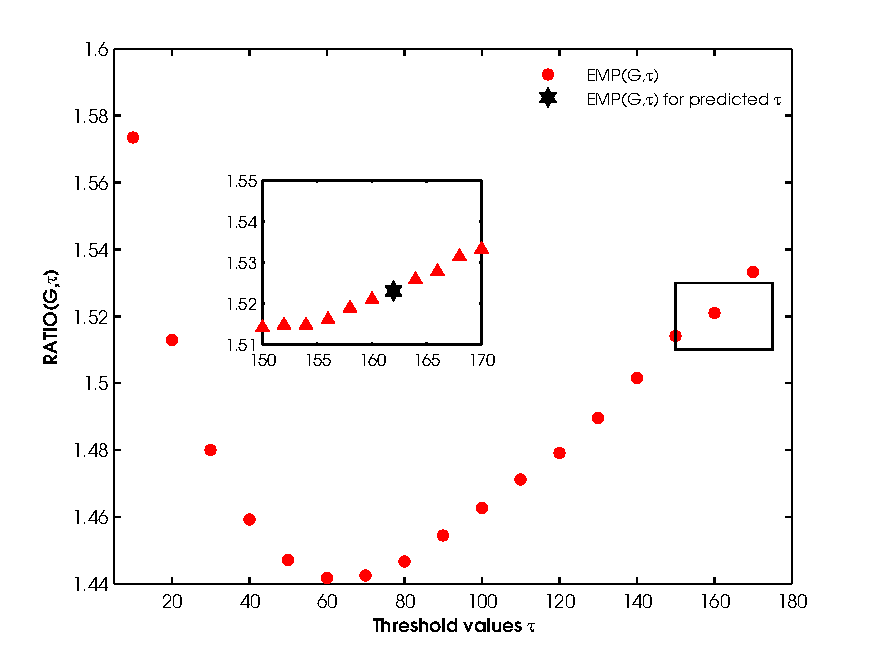
\includegraphics[width=0.5\textwidth]{Figures/enron-ratio.pdf}
%}
%\quad
%\subfloat[\small \textsc{internet}]{
%    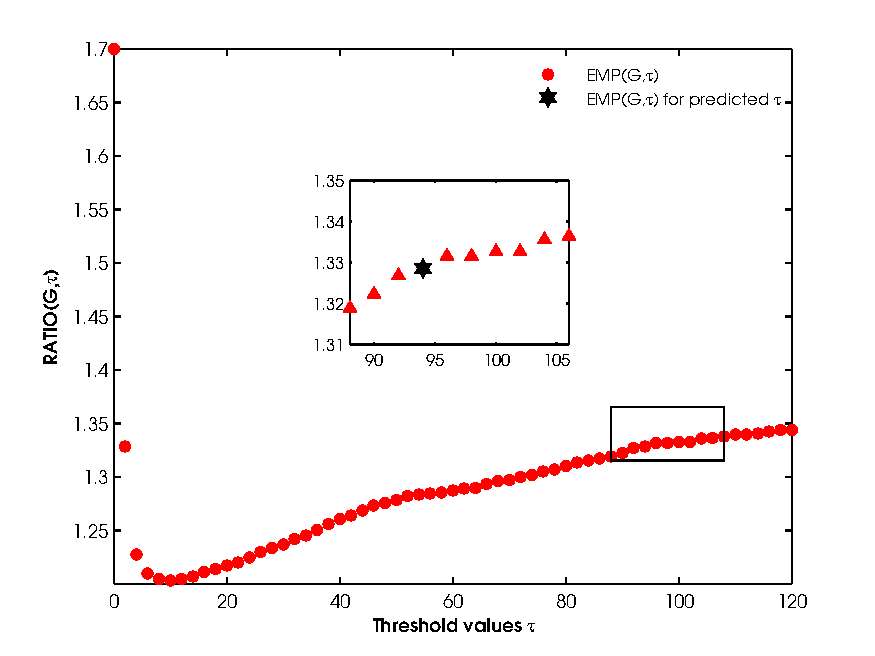
\includegraphics[width=0.5\textwidth]{Figures/internet-ratio.pdf}
%}%
%\caption{Ratios for the real-life datasets \textsc{www}, \textsc{enron} and \textsc{internet}}%
%\label{fig:empdataratios}%
%\end{figure}
%
%\subsection{Stability of power law distribution under different cutoffs}\label{App:ExpRes:Sta}
%In this section we  give an experimental  evidence  that for the synthetic data-sets the distribution of label sizes by itself follows a power-law distribution for any cutoff chosen.
%The label sizes naturally grow, but do so while preserving the power law distribution.
%\begin{figure}[!ht]
%\centering
%\subfloat[\small Cutoff = $5$]{
%    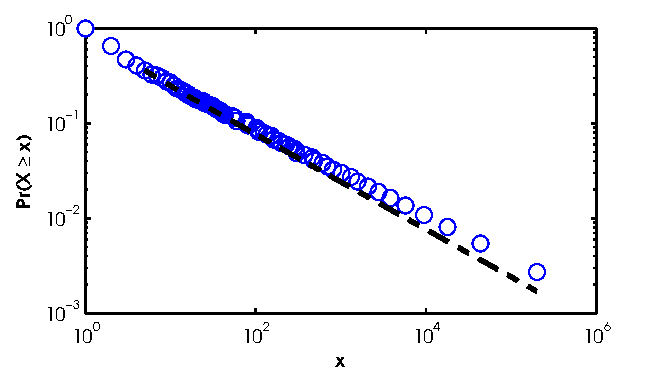
\includegraphics[width=0.33\textwidth]{Figures/alpha/synthetic-data-cutoff5.pdf}
%}%
%\subfloat[\small Cutoff = $30$]{
%    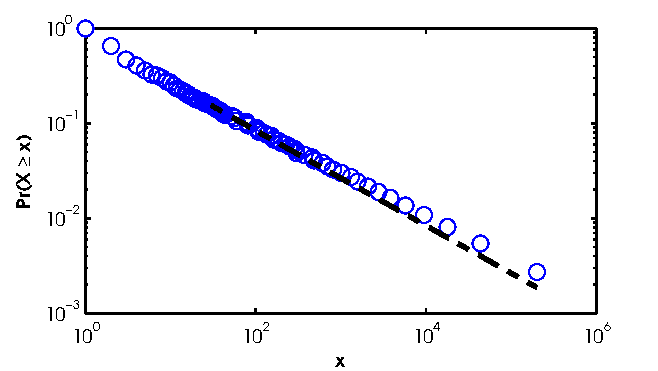
\includegraphics[width=0.33\textwidth]{Figures/alpha/synthetic-data-cutoff30.pdf}
%}%
%\subfloat[\small Cutoff = $1000$]{
%    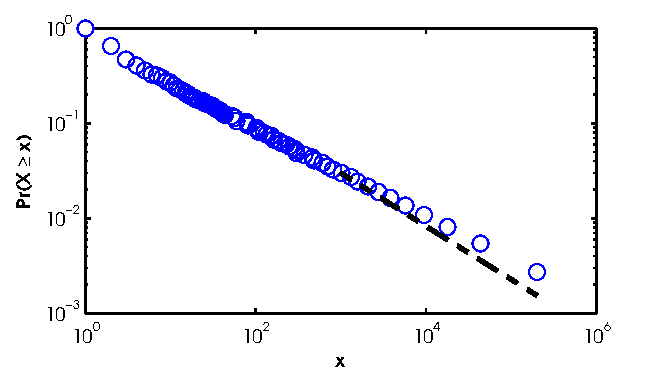
\includegraphics[width=0.33\textwidth]{Figures/alpha/synthetic-data-cutoff1000.pdf}
%}%
%\caption{Best-fitting power law ($\alpha = 2.2$) fitted to the probability mass function of the maximum label sizes for the s300$^{\alpha=2.2}$ dataset using different cutoffs. Power law fit plotted on top of the complementary cumulative distribution function (CCDF) using the framework by \cite{clauset2009power}.} %
%\label{fig:alphavals}%
%\end{figure}





